\documentclass[10pt,letterpaper]{article}
\usepackage{fullpage}
\usepackage{xcolor}
\usepackage{booktabs}
\usepackage{csvsimple}
\usepackage[top=1in, bottom=1in, left=1in, right=1in]{geometry}
\usepackage{graphicx}
\usepackage{wrapfig}
\usepackage{hyperref}
\usepackage{booktabs}
\usepackage{multirow}
\usepackage{amsmath}
\usepackage{subcaption}
\usepackage{algorithm}
\usepackage{algpseudocode}
\usepackage{listings}
\usepackage{xcolor}

\newcommand{\todo}[1]{\textcolor{red}{TODO:\ #1}}
\newcommand{\shortname}{EqMap}

\title{ECE6745 Project -- ASIC Technology Mapping with E-Graphs}
\author{Matthew Hofmann}
\date{\today}

\begin{document}

\maketitle

% Revised Sections
% Introduction
% Background (lit review)
% Baseline design

\section{Introduction}\label{sec:intro}
\subsection{Motivation}\label{sec:intro:motivation}

As transistor scaling comes to a close, the QoR (quality of results) of EDA
tools will become more of a bottleneck in the hardware design process. Given
new developments in compiler technology and automated reasoning tools, it is
possible to better study the suboptimality of the conventional EDA tool stack.
Several of the heuristics used in core EDA algorithms were invented decades
ago, and increases in compute capacity in the modern era afford us a more
formal and exploratory approach to optimizing digital logic. In this project, I
use the automated reasoning capabilities of equality graphs (e-graphs) to more
precisely explore optimal designs points in the PPA (power, performance, area)
trade-off space. With my results, I demonstrate that e-graph driven compilers
can better span the wide gap between SAT-based, exact synthesis and fully
heuristic algorithms.

\subsection{Project Overview}\label{sec:intro:proposal}

Over the length of this course project, I have developed a tool which uses
e-graphs to superoptimize ASIC technology mapping. Besides developing the core
optimization and mapping framework, I have developed a Verilog parser and
emitter to be able to test my technique against existing RTL tools. In short, I
will be comparing against Synopsys Design Compiler. Across 96 RTL benchmarks,
my tool, called \shortname{}, should be able to more exactly synthesize
combinational logic to standard cells. My goal was roughly 10\% area savings
without increasing the circuit depth. Ultimately, I did not reach this goal,
but the results are a promising start. My tool (1) produces \textit{verified}
netlists, (2) often achieves better timing than Synopsys, and (3) is at least
competitive with respect to area.

I was optimistic that my tool could outperform Synopsys on small designs,
because e-graphs can explore circuit topologies that heuristic methods cannot.
However, the real challenge lies within the e-graph extraction algorithm.
Circuit minimization in general in NP-hard, and this problem in my flow
manifests in the extraction stage (Sec.~\ref{sec:alt:extraction}). For this
reason, future work should consider optimizing for delay as it might be more
feasible than optimizing for area. Future experiments will be relatively low
cost to start, because I have a lot of compiler infrastructure already built
up. For instance, I have a custom, bare-bones Verilog frontend. In the
following sections, I will give the literature review needed to understand
equality graphs for superoptimization as well as ASIC technology mapping in
general.

\section{Literature Review}\label{sec:background}

\subsection{E-Graphs}\label{sec:background:egraph}

Equality graphs, most commonly referred to as \textit{e-graphs}, are an
automated reasoning tool built around a union-find data
structure~\cite{eggpaper}. An e-graph is essentially a directed graph with two
extra features: (1) nodes are grouped together into \textit{e-classes} and (2)
edges always start at a node and point to an e-class. As a consequence,
e-graphs can very compactly store a collection of equivalence relations. The
prototypical example for e-graphs involves the rewriting of arithmetic
expressions. For instance, one relation conveyed in Fig.~\ref{fig:egraph} is
that \texttt{a << 1} is equal to \texttt{a * 2}. To convey equality, the
anchoring nodes \texttt{<<} and \texttt{*} are grouped in the same e-class (the
dotted box). However, it is important to note that the destination of edges is
always an e-class and not a node. With this illustration, it hopefully becomes
clear why e-graphs are strong at equational reasoning.

\begin{wrapfigure}{r}{0.47\textwidth}
    \centering
    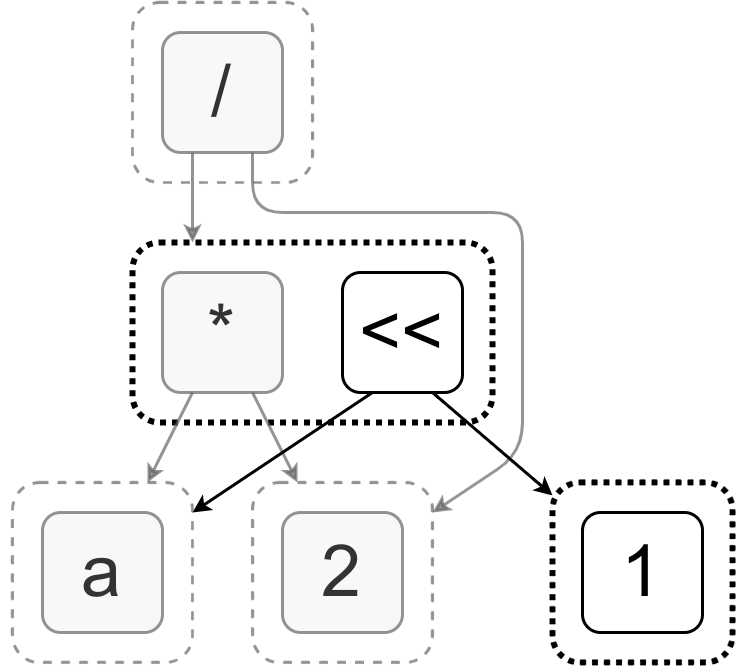
\includegraphics[width=0.44\textwidth]{img/egraph.png}
    \caption{An e-graph with 5 e-classes and 6 e-nodes.}\label{fig:egraph}
\end{wrapfigure}

To give some practical examples, e-graphs have been used to rewrite
mathematical expressions~\cite{egraphmath} or for automated reasoning about
functional programs~\cite{cclemma}. In the case of EDA software, e-graphs can
drive logic synthesis by exploring other circuit topologies. Initially, each
circuit node starts alone in its equivalence class. Then, a set of rewrite
rules is used to grow the e-graph with alternative representations. When
rewrite rules no longer introduce new information into the graph, we say we
have reached \textit{equality saturation}.

Of course, optimizing technology mapping for area is still an NP-hard problem.
E-graphs defer the difficult problem of finding the `best' circuit into a phase
called \textit{extraction}. This is where heuristics are re-introduced. There
are several research projects on e-graph
extraction~\cite{smoothe,sparsextract}, but they are beyond the scope of this
course project. However, previous work on FPGA technology mapping has
demonstrated that fast, greedy extraction algorithms can be used and still find
area and circuit depth improvements. Previous work~\cite{esyn} has demonstrated
the usefulness of e-graphs for logic synthesis. Moreover, I hope to submit my
own e-graph work to ICCAD which shows 12\% area savings over vendor tools on
FPGA applications without increasing circuit depth.

\subsection{ASIC Technology Mapping}\label{sec:background:techmapping}

The standard-cell design methodology for semiconductors came to fruition in the
1980s and 90s. While ASIC design as a general technique is more manageable than
full-custom layouts, there are still provably difficult problems in the flow.
In general, Boolean logic minimization is NP-hard, and this carries over to
architecture-specific problems, i.e., technology mapping. Technology mapping is
the compilation step which converts the abstract RTL logic into a network of
design elements that belong to the standard cell library. In other words, the
input is the user-written logic and the output is a gate netlist. Since exact
technology mapping is hard, most logic synthesis tools are largely driven by
heuristics---either for minimizing area or delay. For instance,
Lily~\cite{areamap} takes into account the connectivity of a circuit in order
to reduce area dedicated to routing signals. Another is example is
how~\cite{powermap} maps cells while taking into account signal transition
probabilities in order to minimize power. Recent developments include works
that use more approximate methods to drive synthesis. For example,
ALS~\cite{approxmap} uses reinforcement learning to do a form of `lossy' logic
synthesis. In my project, I will mostly perform area optimization by tracking
cell counts.

\section{Baseline Compiler Design}\label{sec:baseline}

In the initial design of the compiler, I have developed a logic rewriting
system and an extraction technique that can potentially achieve lower area than
Synopsys Design Compiler. In the case of FPGA technology mapping, I already
have results that show 12\% area savings over the vendor tools without
degrading timing. While greedy extraction shows promise for FPGA applications,
it may be that the same extraction algorithm will be less optimal for ASIC
design. Nonetheless, I anticipate that future work on e-graph extraction
algorithms will improve the circuit synthesis abilities without having to
update the rewriting system. Hence, the logic rewriting system proposed in this
work should be reusable in the future.

\subsection{Boolean Logic Rewriting}\label{sec:baseline:rewriting}
In any case, we can begin to break down the components of the \shortname{}
compiler. First, we need to define the intermediate representation of the
combinational logic that will be rewritten. We can use Backus-Naur form
(BNF)\footnote{\href{https://en.wikipedia.org/wiki/Backus\%E2\%80\%93Naur\_form}{https://en.wikipedia.org/wiki/Backus-Naur\_form}}
to very concisely define the grammar of our intermediate representation of
Boolean logic:

\begin{verbatim}
<Const> ::= false | true

<Input> ::= <String>

<StdCell> ::= NAND_X1 | NOR_X1 | XOR2_X1 | ...

<Node> ::= <Const> | <Input> | (INV <Node>) | (AND <Node> <Node>) | (OR <Node> <Node>)
           | (<StdCell> <Node> <Node>) | (<StdCell> <Node> <Node> <Node>) | ...
\end{verbatim}

Given this very simple language, we can represent any Boolean circuit we want.
For example, we could represent a 2:1 multiplexer with the following syntax:
\texttt{(OR (AND a s) (AND b (INV s)))}. Given this language with formal
semantics, we can write all the properties of Boolean algebras as rewrite
rules. Table.~\ref{tab:rules} shows that there are 19 logic rewriting rules in
total. For more information on the completeness of these rules, one should read
more into the axiomatization of Boolean algebras
\footnote{\href{https://en.wikipedia.org/wiki/Boolean\_algebra\_(structure)\#Axiomatics}{https://en.wikipedia.org/wiki/Boolean\_algebra\_(structure)\#Axiomatics}}.

\begin{table}[h]
    \centering
    \begin{tabular}{cl}
        \toprule
        \textbf{Property}                 & \textbf{Rules}                                         \\ \midrule
        \multirow{2}{*}{Short-Circuit}    & \texttt{(OR a true) => true}                           \\
                                          & \texttt{(AND a false) => false}                        \\ \midrule
        \multirow{2}{*}{Annulment}        & \texttt{(OR a false) => a}                             \\
                                          & \texttt{(AND a true) => a}                             \\ \midrule
        \multirow{2}{*}{Commutativity}    & \texttt{(OR a b) => (OR b a)}                          \\
                                          & \texttt{(AND a b) => (AND b a)}                        \\ \midrule
        \multirow{2}{*}{Associativity}    & \texttt{(OR (OR a b) c) => (OR a (OR b c))}            \\
                                          & \texttt{(AND (AND a b) c) => (AND a (AND b c))}        \\ \midrule
        \multirow{2}{*}{Distributivity}   & \texttt{(OR a (AND b c)) <=> (AND (OR a b) (OR a c))}  \\
                                          & \texttt{(AND a (OR b c)) <=> (OR (AND a b) (AND a c))} \\ \midrule
        \multirow{2}{*}{Complement}       & \texttt{(OR a (INV a)) => true}                        \\
                                          & \texttt{(AND a (INV a)) => false}                      \\ \midrule
        \multirow{2}{*}{De Morgan's Laws} & \texttt{(INV (AND a b)) <=> (OR (INV a) (INV b))}      \\
                                          & \texttt{(INV (OR a b)) <=> (AND (INV a) (INV b))}      \\ \midrule
        \multirow{2}{*}{Idempotence}      & \texttt{(OR a a) => a}                                 \\
                                          & \texttt{(AND a a) => a}                                \\ \midrule
        \multirow{2}{*}{Absorption}       & \texttt{(OR a (AND a b)) => a}                         \\
                                          & \texttt{(AND a (OR a b)) => a}                         \\ \midrule
        Negation                          & \texttt{a => (INV (INV a))}                            \\
        \bottomrule
    \end{tabular}
    \caption{Rules of a Boolean algebra for EqMap}\label{tab:rules}
\end{table}

\subsection{Mapping to Gates}\label{sec:baseline:mapping}

Now that the compiler can reason about Boolean logic, it also needs to know how
to cover the logic with standard cells. We can do this in an ad-hoc fashion by
using rewrite rules to match to syntactical elements in the logic. For example,
the rule \texttt{(INV (AND a b)) => (NAND\_X1 a b)} denotes the logic function
of \texttt{NAND\_X1} and hence declares what portions of the graph it can
cover. Combining cell mapping with the rules from
Sec.~\ref{sec:baseline:rewriting} means that the e-graph will reason about
logic rewriting and mapping to standard cells simultaneously. Hence, the
e-graph can reason about many alternative mappings in parallel. Of course, the
primary trade-off is the memory and execution time needed to build the e-graph.
In any case, Table~\ref{tab:cells} contains an incomplete list of standard
cells and their logic functions in terms of the EqMap intermediate language.

\begin{table}[h]
    \centering
    \begin{tabular}{ll}
        \toprule
        \textbf{Logic Function}                  & \textbf{Standard Cell}                                             \\ \midrule
        \texttt{(INV a)}                         & \texttt{INV\_X1}, \texttt{INV\_X2}, \texttt{INV\_X4}, \ldots       \\
        \texttt{(INV (AND a b))}                 & \texttt{NAND2\_X1}, \texttt{NAND2\_X2}, \texttt{NAND2\_X4}, \ldots \\
        \texttt{(INV (OR a b))}                  & \texttt{NOR2\_X1}, \texttt{NOR2\_X2}, \texttt{NOR2\_X4}, \ldots    \\
        \texttt{(INV (AND (AND a b) (AND c d)))} & \texttt{NAND4\_X1}, \texttt{NAND4\_X2}, \texttt{NAND4\_X4}, \ldots \\
        \texttt{(INV (OR (AND a b) c))}          & \texttt{AOI21\_X1}, \texttt{AOI21\_X2}, \texttt{AOI21\_X4}, \ldots \\
        \texttt{(INV (AND (OR a b) c))}          & \texttt{OAI21\_X1}, \texttt{OAI21\_X2}, \texttt{OAI21\_X4}, \ldots \\
        \bottomrule
    \end{tabular}
    \caption{An incomplete table of cells defined as rewrite rules}\label{tab:cells}
\end{table}

\begin{wrapfigure}{r}{0.47\textwidth}
    \vspace{-1cm}
    \centering
    \includegraphics[width=0.44\textwidth]{img/celllang.pdf}
    \caption{The compilation steps internal to \shortname{} Verilog tool.}\label{fig:flow:egraph}
\end{wrapfigure}

\subsection{Standard Cell Extraction}\label{sec:baseline:extraction}
Ideally, the e-graph is grown until rewrites no longer introduce new terms into
the graph. In the literature, this is called \textit{equality saturation}. In
practice, equality saturation takes too long, and empirically it is not
required to capture the majority of the optimization potential. The quality of
results are more so dependent on the extraction technique used. As explained in
Sec.~\ref{sec:background:egraph}, \textit{extraction} is the process of
selecting the ``best'' circuit from the e-graph. Given that e-graph can easily
contain hundreds of thousands of e-nodes across tens of thousands of e-classes,
a greedy extraction algorithm is the most pragmatic. The greedy extractor
iterates over the e-classes, updating the cost of the cheapest e-node until the
database of costs no longer change. In the baseline compiler, the cost model
simply counts the number of cells required to implement a logic function. For a
circuit node \texttt{x}, its cost is defined as follows:

\begin{figure}[h]
    \[
        F(\texttt{x}) = \begin{cases}
            0                                         & \text{if \texttt{x} is an \texttt{Input} or \texttt{Const}}        \\
            1 + \sum_{\texttt{c} \in C} F(\texttt{c}) & \text{if \texttt{x} is a standard cell with a set of children } C, \\
            \infty                                    & \text{if \texttt{x} is a not a \texttt{StdCell}}.
        \end{cases}
    \]
    \caption{The cost function is defined recursively. The \texttt{INV}, \texttt{AND}, \texttt{OR} node types are purely for logic rewriting, and hence have a cost of infinity to facilitate filtering these choices out of extraction.}\label{fig:cost}
\end{figure}

\subsection{Verilog Integration}\label{sec:baseline:backend}

In order to run meaningful experiments with \shortname{}, I needed to be able
to interface with existing RTL tool flows. This means building some sort of
Verilog compiler from scratch. A half-baked attempt may use a separate tool to
convert the Verilog to a more primitive format---perhaps an and-inverter graph
(AIG). However, it is very important that all compilation stages stay in main
memory if we want a speedy tool. For example, some Verilog test cases are
50,000 lines of code. If we have multiple stages of serialization and parsing,
the performance of the compiler is doomed.

As a starting point, I use the \texttt{sv-parser} Rust crate. This parses the
Verilog and returns an abstract syntax tree (AST). Obviously, reusing a
full-featured Verilog parser is a tremendous amount of work saved. Nonetheless,
an AST is still far from having a compiled Verilog circuit. The AST simply
represents the structure of the input language, not the digital circuit itself.
All that is to say that compiling from an AST data structure is still a lot of
work. In total, I have around 2,000 lines of code dedicated to Verilog
compilation and emission. The entire codebase is creeping into 10,000 lines of
code. Fig.~\ref{fig:flow:egraph} shows the core steps of the compiler. First,
Verilog is compiled to the intermediate representation defined in
Sec.~\ref{sec:baseline:rewriting}. Then, the e-graph is generated with the
rewrite rules. Finally, the `best' circuit is extracted with the cost function
from Fig.~\ref{fig:cost} and it is converted back to Verilog. This enables
nearly seamless integration with other RTL-based tool flows.

\begin{figure}[h]
    \begin{subfigure}{\textwidth}
        \centering
        \includegraphics[width=\textwidth]{img/gates.pdf}
        \caption{The result when mapping a 2-bit CLA to gates of fan-in 2}\label{fig:test:gates}
    \end{subfigure}\vspace{0.5cm}
    \begin{subfigure}{\textwidth}
        \centering
        \includegraphics[width=0.75\textwidth]{img/cells.pdf}
        \caption{EqMap reduces the cell count from 10 to 6 when OAI cells are introduced}\label{fig:test:cells}
    \end{subfigure}
    \caption{Diagrams of the top-level integration of \shortname{} into existing tool flows and internal e-graph driven compiler architecture.}\label{fig:flow}
\end{figure}

Since building out the compiler is the first priority, very little evaluation
was performed at this point. However, the baseline compiler still has
compelling results for simple cases. As an example, the baseline compiler was
tested against a 2-bit carry lookahead unit. Part of the advantage of EqMap is
the flexibility of choosing which library to map to. For example,
Fig.~\ref{fig:test:cells} shows the advantage of introducing OAI and AOI cells
into the library. The mapping uses four less cells than
Fig.~\ref{fig:test:gates}.

\section{Alternative Compiler Design}\label{sec:alt}

The purpose of the baseline design was to have a Verilog-to-Verilog compiler
that could do some basic mapping of AND, OR, and INV logic to the standard
cells used in the course. The alternative design enhances the mapping
capabilities in the hopes that my tool might be able to compete with existing
tools like
Yosys\footnote{\href{https://github.com/YosysHQ/yosys}{https://github.com/YosysHQ/yosys}}
or Synopsys Design Compiler. This meant implementing more cells, as well as
relating existing heuristics for technology mapping to e-graph rewriting and
extraction.

\subsection{More Cells}\label{sec:alt:cells}

In the baseline design of the compiler, only a limited amount of custom cells
in the library were implemented. Now that the end-to-end integration is
complete, it is time to expand the functionality of the flow. Since there are
so many variations of each cell type, it is cumbersome to translate every cell
type into a rewrite rule. This is perhaps the one task I would entrust to an
LLM. However, I still wrote the reasoning rules for the rest of the cells by
hand by reading \texttt{stdcells.v} from the Nangate 45nm Free PDK. The main
cells missing from the baseline design are XOR gates, multiplexers, and
majority gates. There are also many alternate version of AOI and OAI gates,
ranging from 3 to 5 inputs, that were finally implemented. One interesting
thing I learned is that a majority gate is a special case of
\texttt{AOI222}\footnote{\href{https://en.wikichip.org/wiki/majority\_gate\#MAJ3}{https://en.wikichip.org/wiki/majority\_gate\#MAJ3}}.
Tab.~\ref{tab:morecells} shows the rewrite rules for some of the new cells that
were added in the latest iteration of the compiler.

\begin{table}[h]
    \centering
    \begin{tabular}{ll}
        \toprule
        \textbf{Logic Function}                            & \textbf{Standard Cell}                                                \\ \midrule
        \texttt{(INV (OR (OR (AND c1 c2) a) (AND b1 b2)))} & \texttt{AOI221\_X1}, \texttt{AOI221\_X2}, \texttt{AOI221\_X4}, \ldots \\
        \texttt{(INV (AND (AND (OR c1 c2) a) (OR b1 b2)))} & \texttt{OAI221\_X1}, \texttt{OAI221\_X2}, \texttt{OAI221\_X4}, \ldots \\
        \texttt{(OR (AND (INV s) a) (AND s b))}            & \texttt{MUX2\_X1}, \texttt{MUX2\_X2}                                  \\
        \texttt{(INV (AND (AND a b) c))}                   & \texttt{NAND3\_X1}, \texttt{NAND3\_X2}, \texttt{NAND3\_X4}, \ldots    \\
        \texttt{(OR (AND b (INV a)) (AND a (INV b)))}      & \texttt{XOR2\_X1}, \texttt{XOR2\_X2}, \texttt{XOR2\_X4}, \ldots       \\
        \texttt{(OR (AND a b) (OR (AND a c) (AND b c)))}   & \texttt{MAJ3\_X1}, \texttt{MAJ3\_X2}, \texttt{MAJ3\_X4}, \ldots       \\
        \bottomrule
    \end{tabular}
    \caption{An incomplete table of cells defined as rewrite rules}\label{tab:morecells}
\end{table}

\subsection{Exact Area Model}\label{sec:alt:area}

\begin{figure}[h!]
    \centering
    \begin{lstlisting}[language=c++, caption={Cell Area Cost Function}, label={lst:area-code}]
        /// Returns the area of a 45nm cell in um^2.
        pub fn get_min_area(&self) -> Option<f32> {
            match self {
                Self::AND2 => Some(1.064),
                Self::AND3 => Some(1.33),
                Self::AND4 => Some(1.596),
                Self::AOI21 => Some(1.064),
                Self::AOI22 => Some(1.33),
                Self::AOI211 => Some(1.33),
                Self::AOI221 => Some(1.596),
                Self::AOI222 => Some(2.128),
                // ...
                Self::OAI211 => Some(1.33),
                Self::OAI221 => Some(1.596),
                Self::OAI222 => Some(2.128),
                Self::OR2 => Some(1.064),
                Self::XNOR2 => Some(1.596),
                Self::XOR2 => Some(1.596),
                _ => None,
            }
        }
    \end{lstlisting}
    \caption{A Rust function that returns the area of a 45nm cell in $\mu\text{m}^2$.}
\end{figure}

\begin{figure}[h!]
    \[
        F(\texttt{x}) = \begin{cases}
            0                                                                   & \text{if \texttt{x} is an \texttt{Input} or \texttt{Const}}        \\
            \texttt{x.get\_min\_area()} + \sum_{\texttt{c} \in C} F(\texttt{c}) & \text{if \texttt{x} is a standard cell with a set of children } C, \\
            \infty                                                              & \text{if \texttt{x} is a not a \texttt{StdCell}}.
        \end{cases}
    \]
    \caption{The update cost function for greedy extraction using area, instead of cell count.}\label{fig:costa}
\end{figure}

One implementation task in the alternative design was to implement an area cost
model based on the standard cell library \texttt{lib} file. It contains the
area of each gate in units of $\mu\text{m}^2$. In the Rust code, the area
function is implemented as a huge match statement like in
Listing.~\ref{lst:area-code}. Then, this function is passed to the updated
greedy cost metric as shown in Fig.~\ref{fig:costa}.

\subsection{Heuristics Supplanted by Automated Reasoning}\label{sec:alt:heuristics}

The alternative design of the compiler sets out to improve upon the heuristic
techniques we learned from lecture. In particular, I will be drawing points of
comparison and contrast with the course book~\cite{coursebook}. The goal is to
show that unifying technology mapping under an automated reasoning framework
greatly reduces the complexity of implementation and also increases the
resilience of the technology mapper to structural bias. The hypothesis is that
an e-graph driven technology mapper will be less dependent on the
formulation/grouping of the logic terms. That being said, I will now relate the
heuristics from the book~\cite{coursebook} with my implementation: \bigbreak{}
\noindent \textbf{Tree Covering Approximation of DAG Selection.} To make the
technology mapping problem tractable, the book proposes that the DAG
representing the digital circuit be broken down into a forest of trees. As a
consequence, the technology mapper is limited in the ways it can restructure
the logic. In the case of e-graphs, this issue reoccurs, but in a reduced form.
We can rewrite and map the logic with the full DAG structure. However,
extraction is the phase in which this approximation/heuristic could be
re-introduced. For example, greedy extraction will not accurately measure cost
with respect to fan-out. It measures cost as if the graph is a tree. Hence, it
shares the same issue as pointed out in the book. However, if we reformulate
the e-graph extraction problem in terms of mixed-integer linear programming
(MILP) we can find the exact area-optimal solution. There is no escaping the
NP-hardness of the mapping problem, but the e-graph offers more flexibility by
isolating this issue in the extraction phase. \bigbreak{} \noindent
\textbf{Simple Gate Decomposition.} Large fan-in gates that have simple
decompositions are broken down into reduction trees in order to discover more
mappings. This heuristic is partially dependent on the input logic format. For
example, this would be a requirement if the input to your mapper was an
and-inverter graph (AIG). Again, the e-graph here affords lots of flexibility
of input format, and it will automatically explore different reduction tree
topologies as a consequence of the rewrite rule system. In fact, the
commutativity and associativity rules mean \textit{all} the tree decompositions
will be explored. This is a delicate issue to explain, but restructuring the
input logic is vital to mitigating structural bias and this is the main
hypothesized advantage of using automated reasoning for logic synthesis.
\bigbreak{} \noindent \textbf{Inserting Inverter Pairs.} By inserting redundant
inverters in the circuit, the technology mapper can try many more covers of the
graph. For example, observe how De Morgan's laws can be used to interchange
between AND and OR gates. This has an exact analogous feature in the e-graph
rewriting system. More specifically, it is the interaction between the De
Morgan rules and negation rules in Tab.~\ref{tab:rules}. \bigbreak{} \noindent
\textbf{Matching Small DAGs.} The book acknowledges that not all problems can
be solved by partitioning the DAG circuit into a forest of trees. Even very
simple operations like XOR are incompatible with those constraints. Hence, the
book proposes that small structures should use a matching technique to map
those structures outside the general dynamic programming problem. The downside,
however, is this means that those operations further segment the graph into
smaller trees. With e-graph rewriting, this is simply not an issue as we can
expand the search pattern in the e-graph rewrite rule arbitrarily. Of course,
more complex patterns incur more execution time. However, this has not been an
issue for gates like XOR or MAJ3.

\subsection{Exact Extraction Techniques}\label{sec:alt:extraction}

While the e-graph contains many possible cell coverings of the input logic,
finding the best solution is still hard. While greedy extraction is very fast,
it still views the logic structure as one big tree, meaning it can not use
higher levels of fan-out to reduce area. In this project, I put quite a bit of
effort into exploring other extraction techniques. In general, e-graph
extraction is still an open area of research, and my implementation efforts
just reinforce the difficulty of the problem. \bigbreak{} \noindent
\textbf{Integer Linear Programming (ILP) Formulation.} Like many other problems
that are combinatorial in nature, the technology mapping problem can be reduced
into an ILP formulation. This does not change the brute-force nature of the
technique, but it does provides some perspective on the complexity of the
problem. Moreover, it allows us to plug into to other linear programming
solvers to generate our solution. Sec.~\ref{sec:evaluation} provides some
results using an ILP formulation of e-graph extraction. In short, the results
are negative, because the ILP solver cannot be ran on e-graphs as large as the
ones processed with a greedy extractor. Moreover, the cycles in the e-graph
prove to be a huge challenge for both the ILP formulation and the solving
engine. There is a lot more to share about the ILP extraction efforts. However,
they are pretty technical problems, not relevant to ASIC technology, and would
detract from the rest of the ASIC work in the report. However, I will provide
the ILP formulation of e-graph extraction that my compiler uses. It is inspired
from TenSat~\cite{ilpextract}. Extracting some root e-class $C$ takes on the
form of three linear constraints:

\begin{align}
     & x_i \in \{0, 1\} \;\;\;\;                      & \text{(Binary variables to represent choice of nodes)}            & \\
     & \sum_{i \in C} x_i = 1 \;\;\;\;                & (\text{Choose one node to extract from class } C)                 & \\
     & x_i \leq \sum_{j \in \texttt{Children}(i)} x_j & \text{(Any selected node must have its children implemented too)} & \\
    \nonumber                                                                                                               \\
     & \text{Goal: }                                  & \min \sum x_i \cdot \texttt{Cost}(i)                              &
\end{align}

This ILP problem is formulated automatically after e-graph construction, but
before extraction. We use the Rust crate \texttt{good\_lp} to represent the ILP
problem, and this allows for seamless integration with many ILP solvers, like
CBC\footnote{\href{https://github.com/coin-or/Cbc}{https://github.com/coin-or/Cbc}}
and HiGHS\footnote{\href{https://highs.dev/}{https://highs.dev/}}. The cost
model in this context is the cell area metric from Sec.~\ref{sec:alt:area}.
Finally, there are additional constraints not listed here for preventing
combinational loops. As we will see in Sec.~\ref{sec:evaluation}, ILP
extraction does not scale well to the very large e-graphs my tool generates.
Hence, we need to limit the build size in order to obtain results, introducing
a new trade-off.

\begin{algorithm}[h]
    \caption{Best Logic Expression for E-Class $c$ using Dynamic Programming}
    \label{alg:dynprog}
    \begin{algorithmic}[1]
        \Require $e$ \Comment{The e-graph to be extracted from}
        \Require $table$ \Comment{Table to memoize the best results}

        \Function{BestExpr}{$c$}
        \If{$table$ contains $c$}
        \State \Return $table[c]$ \Comment{Return the memoized result}
        \EndIf
        \State $bestArea \gets \infty$ \Comment{Initialize best cost}
        \State $bestExpr \gets \texttt{None}$ \Comment{Initialize best expression}
        \For{$n$ in \Call{Nodes}{$c$, $e$}} \Comment{Iterate over all nodes in the e-class}
        \If{\Call{Visited}{$n$}} \Comment{Break out of cycles}
        \State \textbf{Continue}
        \EndIf
        \State $bestChildren \gets []$ \Comment{List for best children}
        \For{$v$ in \Call{Children}{$n$}} \Comment{Iterate over child e-classes}
        \State $bestChildren \gets bestChildren\; + $ \Call{BestExpr}{$v$, $e$} \Comment{Append the list with recursive step}
        \EndFor
        \State $candidate \gets$ \Call{Combine}{$bestChildren + n$} \Comment{Combine the sub-circuits into one}
        \If{\Call{Area}{$candidate$} $<$ $bestArea$}
        \State $bestArea \gets$ \Call{Area}{$candidate$} \Comment{Update best cost}
        \State $bestExpr \gets candidate$ \Comment{Update best expression}
        \EndIf
        \EndFor
        \State $table[c] \gets bestExpr$ \Comment{Memoize the result}
        \State \Return $bestExpr$ \Comment{Return the best expression}
        \EndFunction
    \end{algorithmic}
\end{algorithm}

\bigbreak{} \noindent \textbf{Dynamic
    Programming.} We can also use dynamic programming as another way to brute force the solution
to exact technology mapping. The tree covering algorithm as presented in the
course textbook~\cite{coursebook} is optimal, disregarding the DAG partitioning
part. However, extending the same algorithm to e-graph extraction is naive,
because e-graph rewriting also restructures the logic. In other words, the
e-graph extractor needs to compute the best cell covering for every single
possible equivalent graph, whereas the textbook algorithm is given a graph and
only needs to find the best covering for said graph. Obviously, the e-graph
posing of the problem may prove more optimal, but it admits a much wider
solution space to search. Algorithm~\ref{alg:dynprog} shows the dynamic
programming implementation I used. When choosing the best gate mapping for an
e-class $c$, we first recursively find the best gate mappings for all the child
e-classes for all the nodes in the e-class. Then, we combine the circuits using
common sub-expression elimination (the call to \texttt{Combine} in
Alg.~\ref{alg:dynprog}). If the candidate circuit is better than the current
best, we update the best circuit. Finally, a lookup table is used to memoize
the results. The dynamic programming algorithm as presented in the course
textbook does not need a common sub-expression elimination step, because it is
always covering the same graph. On the other hand, the e-graph models all
possible restructuring of the logic according to Boolean algebra. Hence, the
e-graph extractor presents many `best' solutions. As a result,
Alg.~\ref{alg:dynprog} is quick but produces sub-optimal results. I attempted to
augment the algorithm by storing multiple `best' expressions, then checking
them all in a loop. This is the correct fix, but the execution time and spaces
grows factorially. After all, the e-graph contains all Boolean restructuring of
the logic. Since this algorithm only worked on very small e-graphs, there are
no results reported using this technique in Sec.~\ref{sec:evaluation}. However,
I do include some ILP results. In both the case of ILP and dynamic programming,
we see that there are consequences for widening the solution space so much over
more classic technology mapping algorithms. There is no free lunch.

\subsection{Node Pruning}\label{sec:alt:pruning}

To mitigate the scalability problems with the ILP extractor, I added a `node
pruning' step after e-graph building, but before extraction. To provide some
context, I use the logical nodes (\texttt{AND}, \texttt{OR}, \texttt{INV}) to
facilitate e-graph exploration, but they are filtered out during extraction by
giving them $\infty$ cost. This technique works well for the greedy extractor.
However, it cripples the ILP solvers with useless constraints. For brevity's
sake, I will not show the code as it is not very interesting, but you can find
it
here\footnote{\href{https://github.com/matth2k/lut-synth/blob/ece6745/src/driver.rs\#L584}{https://github.com/matth2k/lut-synth/blob/ece6745/src/driver.rs\#L584}}.
However, this pruning step proved vital in obtaining the results in
Tab.~\ref{tab:ilp}. It cut the amount of linear constraints by roughly one
third. Moving forward, I think this a neat feature that can be developed into a
full-on heuristic.

\section{Testing}\label{sec:testing}

Throughout the course of this project, I used a varied testing strategy on both
the software development front and the circuit verification front. For the
project to be successful, it is very important to abstract the components of
the compiler wisely and test them rigorously. This enforces some level of
self-consistency in how the layers of the compiler integrate with each other.
Nonetheless, end-to-end testing is still required to capture the demands of the
end application---having a working Verilog-to-Verilog compiler. Hence, there is
nearly as much testing code as there is compiler code. The full list of testing
strategies is itemized below:

\begin{itemize}
    \item Software Testing
          \begin{itemize}
              \item Unit tests are written with the Rust Cargo tools in mind (\texttt{cargo test}).
              \item 36 end-to-end regression tests are ran with the full Verilog tool flow.
              \item Both of these test types are checked in a GitHub CI workflow.
              \item Results for 99 Verilog benchmarks are continually recorded and new commits are
                    checked for abnormalities.
              \item I self-enforce 80\% code coverage by line on my code.
          \end{itemize}
    \item Circuit Verification
          \begin{itemize}
              \item The intermediate language is its own statically typed data structure. A
                    mini-linter is built around it to check for syntax errors.
              \item Verilator is used to lint Verilog output for sanity checking.
              \item The compiler performs exhaustive testing of combinational logic. Although, this
                    is only feasible for small circuits.
              \item Yosys RTL equivalence checking is used as a third party source to verify the
                    correctness of the Verilog output against the original Verilog input.
              \item The e-graph can produce a proof of the rewrite sequence that relates the
                    optimized and original form of the Verilog.
          \end{itemize}
\end{itemize}

\section{Evaluation}\label{sec:evaluation}

\begin{table}[h]
    \centering
    \caption{ISCAS'85 Benchmark results comparing MSynth (My e-graph driven tool) against Synopsys Design Compiler. Fast, greedy e-graph extraction is used.}\label{tab:results}
    \csvreader[
        tabular=lrrrrrrrrr, % Custom alignment for this instance
        late after line=\\, % Add \\ after each row
        late after last line=\\ \bottomrule, % Prevent extra \\ after the last row
        table head=\toprule Module & Cell Count & & Area ($\mu\text{m}^2$) & & Arrival Time (ns) &  \\ \midrule
    ]{data/results.csv}{1=\one, 2=\two, 3=\three, 4=\four, 5=\five, 6=\six, 7=\seven}%
    {\one & \two & \three & \four & \five & \six & \seven}
\end{table}

\begin{table}[h]
    \centering
    \caption{Results comparing greedy extraction technique with ILP formulation of the extraction problem. The ILP results are worse, because the e-graph needed to be limited in size (8000 nodes), whereas the greedy extractor still works on e-graphs grown to hundreds of thousands of nodes.}\label{tab:ilp}
    \csvreader[
        tabular=lrrrrrrrrr, % Custom alignment for this instance
        late after line=\\, % Add \\ after each row
        late after last line=\\ \bottomrule, % Prevent extra \\ after the last row
        table head=\toprule Module & Area ($\mu\text{m}^2$) & & Extraction Time (s) &  \\ \midrule
    ]{data/ilp.csv}{1=\one, 2=\two, 3=\three, 4=\four, 5=\five}%
    {\one & \two & \three & \four & \five}
\end{table}

Early results are promising, because they demonstrate that e-graph driven
compilers can scale to the thousands of gates. As an example, a 4,000 line
Verilog module with 108 outputs can be expanded to an e-graph with 50,000 nodes
in seconds. Including Verilog compilation and emission, the total synthesis
time is approximately 10 seconds. Of course, we can extend or shorten the
amount of time spent on e-graph construction. Moreover, the results are also
evidence that automated reasoning and the Rust programming language are great
tools for creating robust, high quality compilers. E-graphs force us to define
formal semantics for our Verilog netlists, and Rust's static typing, pattern
matching, and memory safety enforce a certain level of code hygiene. Software
development aside, Yosys is used to perform SAT-based equivalence checking to
verify the resulting netlists. In short, the gate netlists are proven to be
logically equivalent. Tab.~\ref{tab:results} shows early results compiling
benchmarks from the ISCAS'85 suite. These modules span from a handful of number
of gates into the thousands. Likewise, some have very few output ports, while
some have hundreds.

In general, the results of my custom compiler are roughly 1.5x worse with
respect to area. This is because my compiler has not addressed the DAG
selection / tree partitioning problem. Fig.~\ref{fig:dag} shows a very small
circuit which demonstrates the issue. The circuit shows that creating a
\texttt{NAND2} and \texttt{AND2} in parallel is wasteful when they share the
same inputs. However, greedy extraction will produce the sub-optimal solution
in Fig.~\ref{fig:dag:bad}. On the other hand, Fig.~\ref{fig:dag:good} reuses
the \texttt{NAND2} logic and the entire circuit is half the area. While this
example is simple to understand, computing the optimal solution in general is
combinatorial in nature and is proven in general to be NP-hard. In short, exact
circuit selection is computationally intractable. At the same time, the default
greedy extraction algorithm I am using is too primitive. It cannot increase the
fan-out of gates to share computation and save area. Clearly, I will need to
re-implement some heuristics in future work.

\begin{figure}[h]
    \begin{subfigure}{0.48\textwidth}
        \centering
        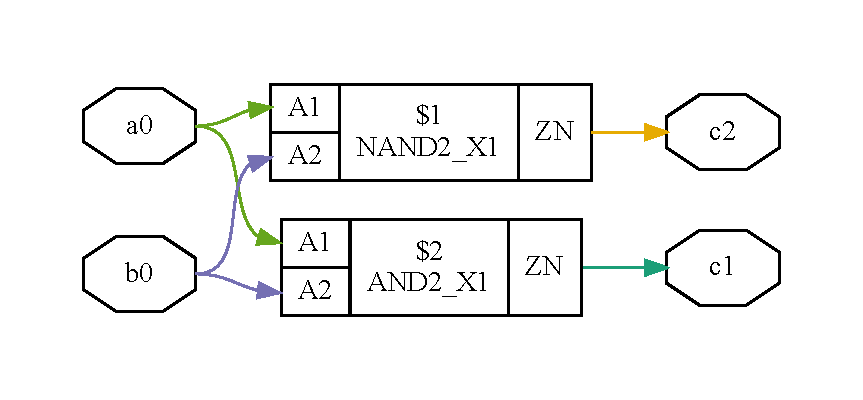
\includegraphics[width=\textwidth]{img/bad.pdf}
        \caption{Using a separate NAND2 and AND2 is redundant.}\label{fig:dag:bad}
    \end{subfigure}
    \begin{subfigure}{0.48\textwidth}
        \centering
        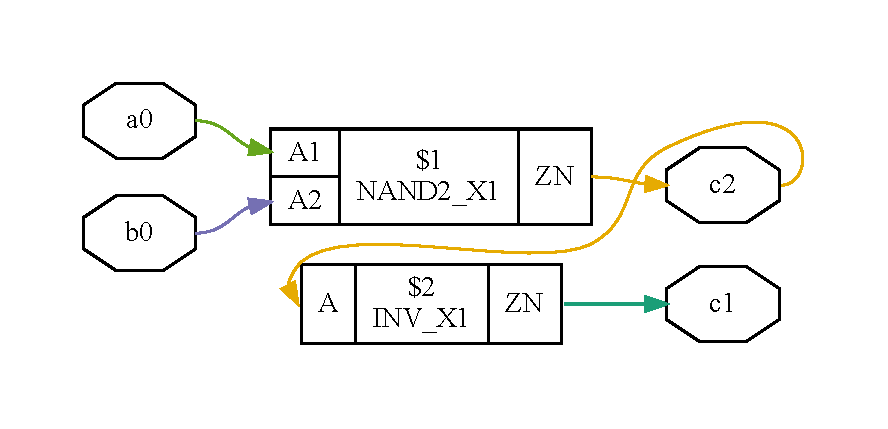
\includegraphics[width=\textwidth]{img/good.pdf}
        \caption{Sharing the NAND2 is much better.}\label{fig:dag:good}
    \end{subfigure}
    \caption{DAG selection in general is an NP-hard problem. Hence, a tree partition heuristic is needed to create higher fan-out gates that share logic.}\label{fig:dag}
\end{figure}

As for timing, my results are much more competitive. In fact, the e-graph
produced netlists have better arrival time in all but two cases. Using c7552 as
an example, the delay path is roughly 33\% shorter when using my compiler over
Synopsys. Lastly, I will address the failure of ILP driven exact extraction. In
short, it is supposed to solve the problem exactly. However, it does not scale
to the e-graphs we want to process. For example, the results in
Tab.~\ref{tab:results} does not restrict the size of the e-graph, and many
e-graphs grew into the hundreds of thousands of nodes. Meanwhile, the ILP
results in Tab.~\ref{tab:ilp} are limited to 8,000 nodes. In the end, it means
we have an extraction time that is roughly 10,000x slower just to achieve a
worse result. Clearly, we need to invent new extraction heuristics. It is an
open area of research~\cite{smoothe,sparsextract,ilpextract}, but there are no
robust Rust implementations of said research that can be integrated and tested
today, without writing more code.

\section{Conclusion and Future Work}\label{sec:conclusion}

In this project, I build an ASIC technology mapping tool that uses
industry-standard Verilog as input and output. While the project proved that
e-graphs for automated reasoning can be used to make verified compilers very
quickly, the argument for higher levels of optimization still needs to be
proven. All my netlists were verified, but the area was roughly 1.5x worse than
Synopsys DC. At the very least, the timing was better in all but two cases.
Future work on extraction remains.

In the future, I plan to also re-implement the tree partitioning heuristic.
Moreover, I plan to continue tweaking my cost model to take into account power
and latency. As for the experimentation, I plan to introduce a second baseline:
Yosys. There are no existing Yosys passes to do the full logic synthesis and
technology mapping for ASIC. I can create my own Yosys pass, but I did not have
enough time for this deadline. Maybe I can also measure switching energy in my
cost model. Lastly, I will run the tools on a larger set of benchmarks, perhaps
Verilog that other students wrote in the course. Within this project, my
extraction technique was too primitive to make it worthwhile to expand to more
benchmarks. I spent the large majority of the last two weeks making ILP
extraction feasible. In the end, I am satisfied with this project, because it
brought in a lot of challenges not presented by the FPGA LUT mapping. These
problems will no doubt be inspiration for future research.

\nocite{*}
\bibliographystyle{plain-annote}
\bibliography{references}

% TODOs:
% - Are Model
% - Talk about ILP
% - Describe dynamic programming algorithm

\end{document}